% 第2章 数据获取与分析

\section{数据获取与分析}

\subsection{数据来源与样本说明}

本文使用的数据来自项目仓库中的\texttt{real\_data\_complete.csv}。样本期覆盖2015年9月28日至2025年12月24日，经滚动窗口构造和缺失值处理后，主样本保留2489个有效观测，其中训练样本1493个，测试样本996个。训练集与测试集完全按时间顺序划分，未进行随机打乱。这样的处理既符合时间序列回归的基本规范，也为样本外评估提供了可比较的基础。

本研究以沪深300指数为研究对象，主要考虑其覆盖面广、流动性好、与中国市场整体运行状态的联动较强。由于研究目标已经从收益率方向转为短期不稳定性，因此数据体系不再依赖大量市场微观字段，而是集中于能够支持波动状态建模的指数价格与月度宏观变量。指数收盘价用于构造日对数收益率，月度宏观变量则用来刻画政策环境、汇率变化、价格信号和货币边际变化。

\subsection{数据整理与预处理过程}

数据预处理遵循统一、简洁和避免前视偏误三项原则。首先，以交易日为基准索引计算日对数收益率\(r_t=\ln(P_t/P_{t-1})\)。随后，利用未来5日与未来20日滚动窗口构造主因变量和辅助因变量。历史状态变量则分别以过去5日、20日和60日平均绝对收益，或其对数实现波动率形式表示。所有由滚动窗口产生的缺失值在样本构造阶段统一剔除。

月度宏观变量对齐采用"上一个完整月可得信息"原则。任一交易日上可使用的宏观变量值，均来自上一个完整月已经可观测的数值。这一规则保证了宏观变量不会提前吸收未来信息。经济政策不确定性指数与汇率变量先取对数或对数差分，再形成月度摘要；PPI同比增速和M2增速月度变化则直接使用对齐后的月度值。

在模型估计层面，训练集和测试集的划分先于任何参数学习过程。标准化只在训练集上拟合，测试集严格沿用训练集参数进行映射。由于正式模型使用的宏观变量维度已明显降低，数据整理阶段不再实施复杂的高维特征筛选，而是把重心放在变量口径的稳定性与回归推断的一致性上。

\subsection{变量分类与核心指标}

本文变量可分为三类。第一类是收益与不稳定性变量，包括日对数收益率\(r_t\)、未来五日平均绝对收益\texttt{future\_absret\_5}、未来二十日实现波动率对数\texttt{future\_logrv\_20}，以及对应的历史状态变量\texttt{past\_absret\_5}、\texttt{past\_absret\_20}、\texttt{past\_absret\_60}与\texttt{past\_logrv\_5}、\texttt{past\_logrv\_20}、\texttt{past\_logrv\_60}。第二类是宏观解释变量，包括\texttt{epu\_log\_m1}、\texttt{fx\_ret1\_m1}、\texttt{ppi\_yoy\_m1}、\texttt{m2\_delta1\_m1}。第三类是辅助评估指标，包括样本内\(R^2\)、调整后\(R^2\)、样本外\(R^2_{OS}\)、RMSE、MAE与若干残差诊断统计量。

在经济含义上，\texttt{future\_absret\_5}刻画的是未来一周平均波动幅度，是本文正式研究中的主因变量；\texttt{future\_logrv\_20}反映的是更平滑的中期波动状态，用于稳健性对照。历史状态变量的设置遵循HAR模型的异质时间尺度思想，分别对应短期、中期和较长期历史不稳定性。宏观解释变量则覆盖政策环境、汇率变化、工业品价格和货币条件四个维度，代表外部背景变量对短期不稳定性的可能影响。

\subsection{描述统计分析}

主因变量\texttt{future\_absret\_5}的均值为0.008443，标准差为0.005026，最小值为0.000761，最大值达到0.059450，偏度为2.7193，峰度为14.3409，显示出显著的右偏和厚尾特征。也就是说，多数时期的短期不稳定性处于较低水平，但在少数阶段会迅速升高并形成较长右尾。辅助因变量\texttt{future\_logrv\_20}的均值为-9.1866，标准差为0.8335，分布明显更平滑，偏度和峰度都较低，适合作为中期状态变量的稳健性对照。

历史状态变量呈现出随窗口拉长而波动收敛的特征。\texttt{past\_absret\_5}与主因变量的均值接近，但标准差较大；\texttt{past\_absret\_20}和\texttt{past\_absret\_60}的标准差依次下降，说明较长窗口下的平均波动状态更平滑。宏观变量中，\texttt{epu\_log\_m1}呈现阶段性台阶变化，\texttt{fx\_ret1\_m1}的均值接近零但波动集中，\texttt{ppi\_yoy\_m1}在样本期内经历了完整的景气循环，\texttt{m2\_delta1\_m1}则围绕零值上下波动。

% 表2-1：主要变量描述统计（收益与不稳定性变量）
\begin{table*}[htbp]
\centering
\footnotesize
\caption{主要变量描述统计（收益与不稳定性变量）}
\label{tab:descriptive-stats-1}
\begin{tabular}{lcccccc}
\topline
变量 & 均值 & 标准差 & 最小值 & 最大值 & 偏度 & 峰度 \\
\midline
\texttt{r\_t} & 0.0001 & 0.0121 & -0.0821 & 0.0814 & -0.474 & 5.924 \\
\texttt{future\_absret\_5} & 0.0084 & 0.0050 & 0.0008 & 0.0594 & 2.719 & 14.341 \\
\texttt{future\_logrv\_20} & -9.1870 & 0.8340 & -11.8900 & -6.7010 & 0.305 & 0.096 \\
\texttt{past\_absret\_5} & 0.0084 & 0.0050 & 0.0008 & 0.0594 & 2.718 & 14.339 \\
\texttt{past\_absret\_20} & 0.0085 & 0.0037 & 0.0021 & 0.0266 & 1.526 & 3.251 \\
\texttt{past\_absret\_60} & 0.0086 & 0.0032 & 0.0035 & 0.0253 & 1.241 & 2.357 \\
\texttt{past\_logrv\_5} & -9.4110 & 1.0530 & -14.1420 & -5.5770 & 0.057 & 0.644 \\
\texttt{past\_logrv\_20} & -9.1860 & 0.8340 & -11.8900 & -6.7010 & 0.305 & 0.093 \\
\texttt{past\_logrv\_60} & -9.0500 & 0.7570 & -10.7060 & -6.7590 & 0.275 & -0.297 \\
\bottomline
\end{tabular}
\end{table*}

% 表2-2：宏观变量描述统计
\begin{table*}[htbp]
\centering
\footnotesize
\caption{宏观变量描述统计}
\label{tab:descriptive-stats-2}
\begin{tabular}{lcccccc}
\topline
变量 & 均值 & 标准差 & 最小值 & 最大值 & 偏度 & 峰度 \\
\midline
\texttt{epu\_log\_m1} & 6.300 & 0.460 & 4.652 & 6.878 & -1.269 & 1.225 \\
\texttt{fx\_ret1\_m1} & 0.0014 & 0.0121 & -0.0273 & 0.0436 & 0.591 & 0.980 \\
\texttt{ppi\_yoy\_m1} & 0.8340 & 4.6190 & -5.9000 & 13.5000 & 0.689 & -0.485 \\
\texttt{m2\_delta1\_m1} & -0.0410 & 0.4940 & -1.6000 & 1.3000 & -0.093 & 0.619 \\
\bottomline
\end{tabular}
\end{table*}

% 图2-1：future_absret_5时间序列图
\begin{figure}[htbp]
\centering
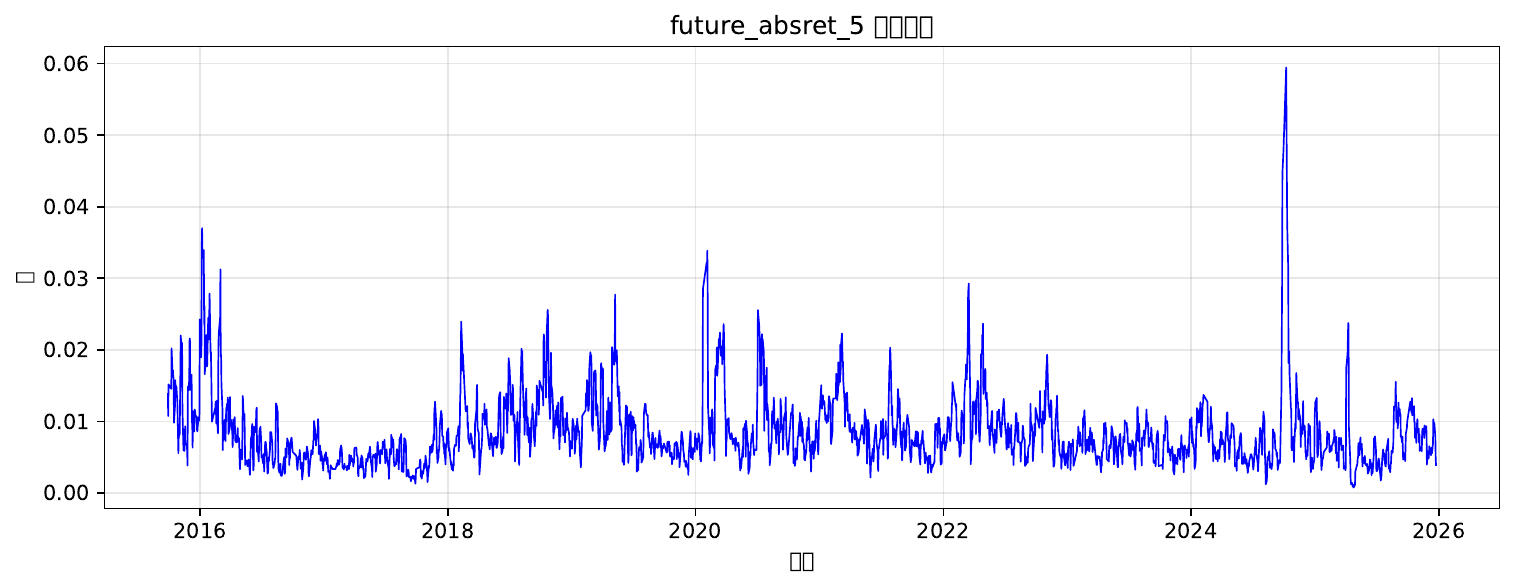
\includegraphics[width=0.85\textwidth]{figures/future_absret_5.png}
\caption{\texttt{future\_absret\_5}时间序列图}
\label{fig:future-absret}
\end{figure}

% 图2-2：future_logrv_20时间序列图
\begin{figure}[htbp]
\centering
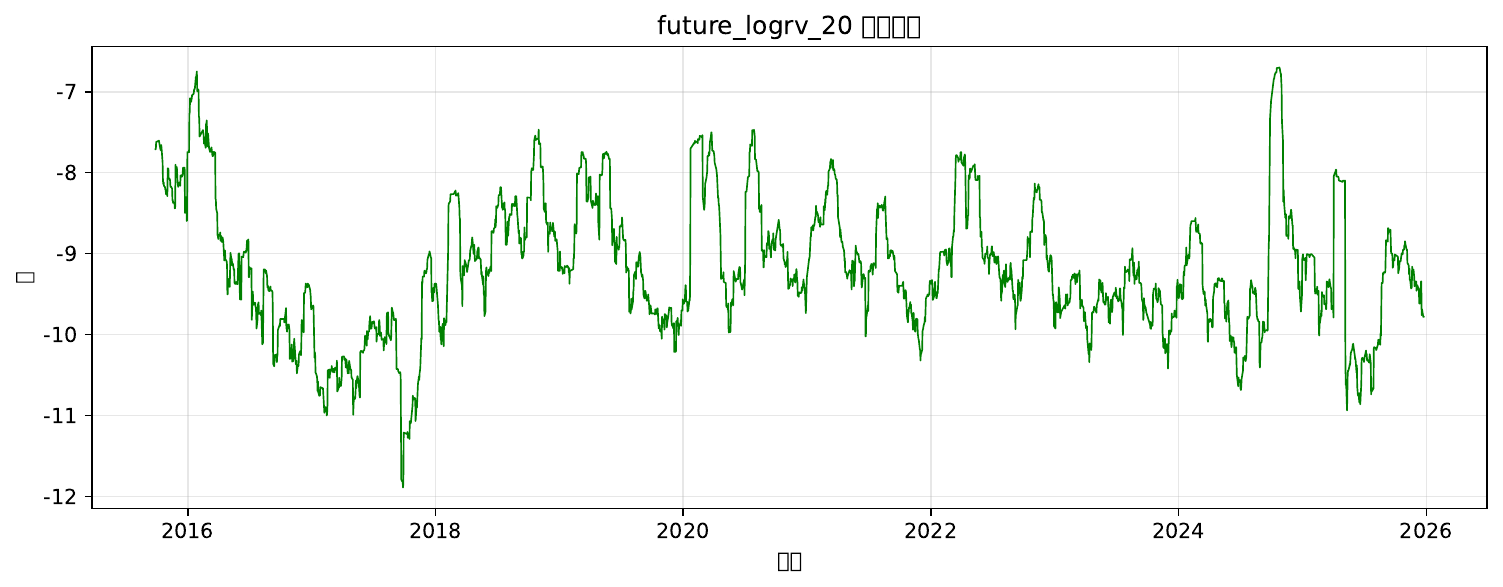
\includegraphics[width=0.85\textwidth]{figures/future_logrv_20.png}
\caption{\texttt{future\_logrv\_20}时间序列图}
\label{fig:future-logrv}
\end{figure}

% 图2-3：宏观变量时间序列图
\begin{figure}[htbp]
\centering
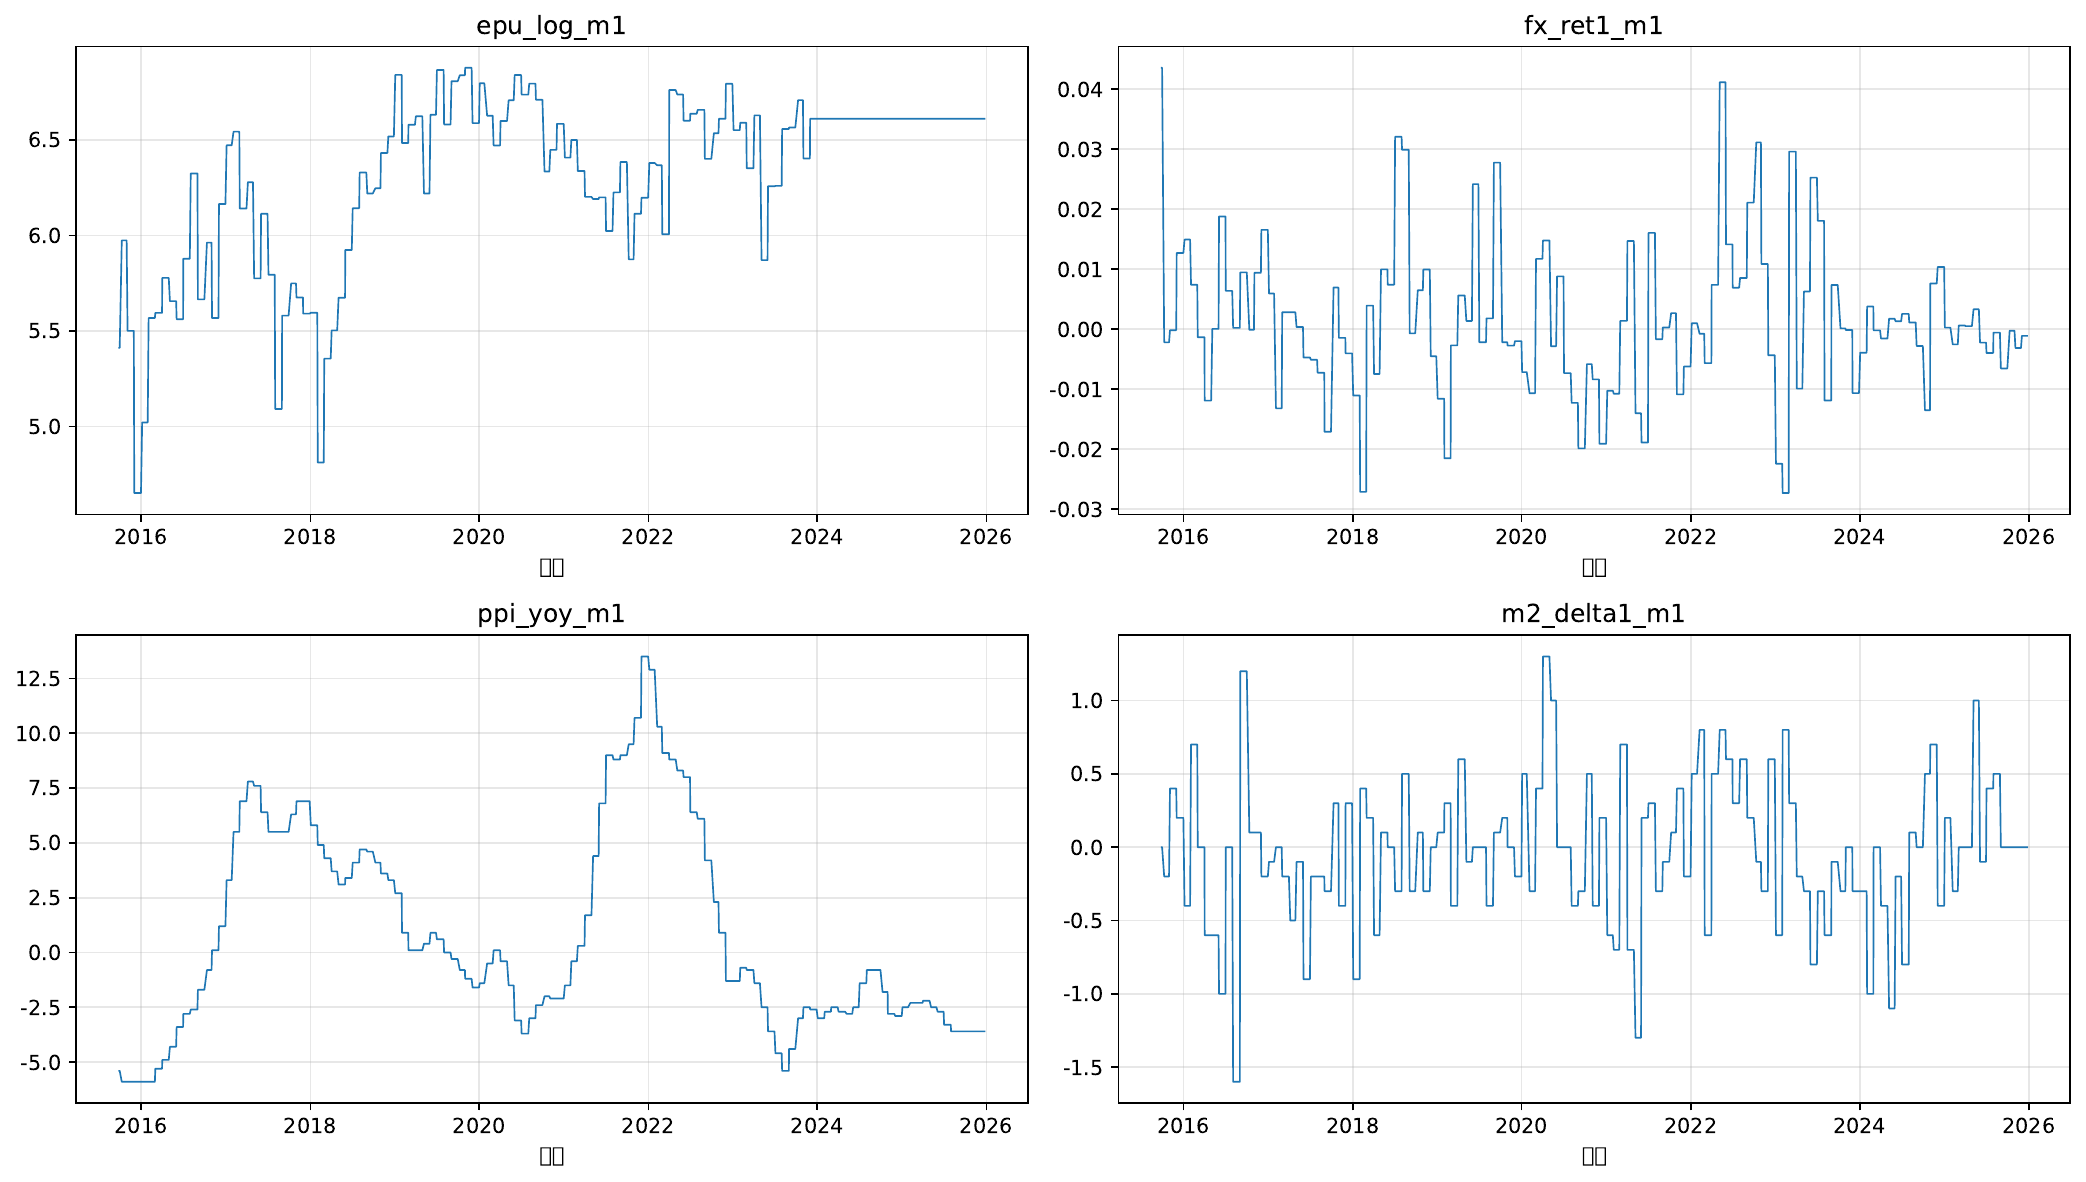
\includegraphics[width=0.85\textwidth]{figures/macro_variables.png}
\caption{宏观变量时间序列图}
\label{fig:macro-series}
\end{figure}

\subsection{相关性与初步关系检验}

相关性分析进一步说明，主因变量的主要信息首先来自历史状态变量本身。\texttt{future\_absret\_5}与\texttt{past\_absret\_5}的相关系数为0.897，与\texttt{past\_absret\_20}的相关系数为0.643，与\texttt{past\_absret\_60}的相关系数为0.444。这个结果非常直观地表明，未来一周平均波动幅度与过去5日和20日历史状态的联系最紧密，而60日尺度虽然仍有相关性，但强度已经明显下降。

与主因变量相比，宏观变量与\texttt{future\_absret\_5}的线性相关性整体较弱。\texttt{epu\_log\_m1}、\texttt{fx\_ret1\_m1}、\texttt{ppi\_yoy\_m1}与\texttt{future\_absret\_5}的相关系数绝对值都不高，这预示了宏观变量在正式回归中更可能表现为边际修正项，而不会成为主导性解释来源。辅助因变量\texttt{future\_logrv\_20}与其对应的\texttt{past\_logrv\_5}、\texttt{past\_logrv\_20}、\texttt{past\_logrv\_60}相关性极高，说明中期波动状态本身具有更强的持续性，这也解释了为何该因变量在样本外评估中表现得极好。

% 表2-3：future_absret_5与HAR状态变量相关系数矩阵
\begin{table*}[htbp]
\centering
\footnotesize
\caption{\texttt{future\_absret\_5}与HAR状态变量相关系数矩阵}
\label{tab:corr-absret}
\begin{tabular}{lcccc}
\topline
变量 & \texttt{future\_absret\_5} & \texttt{past\_absret\_5} & \texttt{past\_absret\_20} & \texttt{past\_absret\_60} \\
\midline
\texttt{future\_absret\_5} & 1.000 & 0.897 & 0.643 & 0.444 \\
\texttt{past\_absret\_5} & 0.897 & 1.000 & 0.693 & 0.468 \\
\texttt{past\_absret\_20} & 0.643 & 0.693 & 1.000 & 0.740 \\
\texttt{past\_absret\_60} & 0.444 & 0.468 & 0.740 & 1.000 \\
\bottomline
\end{tabular}
\end{table*}

% 表2-4：future_absret_5与宏观变量相关系数矩阵
\begin{table*}[htbp]
\centering
\footnotesize
\caption{\texttt{future\_absret\_5}与宏观变量相关系数矩阵}
\label{tab:corr-macro}
\begin{tabular}{lcccc}
\topline
变量 & \texttt{future\_absret\_5} & \texttt{epu\_log\_m1} & \texttt{fx\_ret1\_m1} & \texttt{ppi\_yoy\_m1} \\
\midline
\texttt{future\_absret\_5} & 1.000 & -0.074 & 0.060 & -0.065 \\
\texttt{epu\_log\_m1} & -0.074 & 1.000 & -0.041 & -0.145 \\
\texttt{fx\_ret1\_m1} & 0.060 & -0.041 & 1.000 & 0.034 \\
\texttt{ppi\_yoy\_m1} & -0.065 & -0.145 & 0.034 & 1.000 \\
\bottomline
\end{tabular}
\end{table*}

% 表2-5：future_logrv_20与HAR状态变量相关系数矩阵
\begin{table*}[htbp]
\centering
\footnotesize
\caption{\texttt{future\_logrv\_20}与HAR状态变量相关系数矩阵}
\label{tab:corr-logrv}
\begin{tabular}{lcccc}
\topline
变量 & \texttt{future\_logrv\_20} & \texttt{past\_logrv\_5} & \texttt{past\_logrv\_20} & \texttt{past\_logrv\_60} \\
\midline
\texttt{future\_logrv\_20} & 1.000 & 0.976 & 0.988 & 0.983 \\
\texttt{past\_logrv\_5} & 0.976 & 1.000 & 0.977 & 0.961 \\
\texttt{past\_logrv\_20} & 0.988 & 0.977 & 1.000 & 0.986 \\
\texttt{past\_logrv\_60} & 0.983 & 0.961 & 0.986 & 1.000 \\
\bottomline
\end{tabular}
\end{table*}

\subsection{样本特征总结与对后续模型的支撑}

从数据特征来看，本文的经验分析具备几个明显前提。主因变量存在较强右偏和厚尾，因此需要在回归阶段使用稳健标准误处理潜在异方差。主因变量与HAR历史状态变量之间具有较高相关性，为构建基准动态模型提供了充分依据。宏观变量与主因变量的线性相关性整体不强，说明后续的HARX扩展更适合作为增量检验，而不适合被预设为显著提高样本外表现的模型。辅助目标\texttt{future\_logrv\_20}与历史状态变量的高度相关，则提示其中期状态持续性极强，更适合作为稳健性对照而非主结论来源。
